\begin{frame}{Circle}
{\textbf{Problem:7}\\Let A and B be the centres of two circles of equal radii 3 such that each one of them passes through the centre of the other. Let them intersect at C and D. Is AB $\perp$ CD?}
\begin{itemize}
\item \textbf{Solution:}
\end{itemize}
\textbf{Given:}\\
Radious of circle A = B = 3cm .\\
C and D are the intersecting points.\\
AD = AC and BD = BC.\\
Radius of both circles are equal,\\
 therefore,\\
 AD = AC = BC = BD.\\
then ABCD form a Rhombus and the diagonals of rhombus bisects each other at 90\degree.\\
from the figure  AB $\perp$ CD.\\ 
the python code for  Figure 0-13 is codes/cir\_con.py\\
and the equivalent latex-tikz code for Figure 0-14 is cir\_con.tex
\end{frame}
\begin{frame}{} 
\begin{figure}[!ht]
	\begin{center}
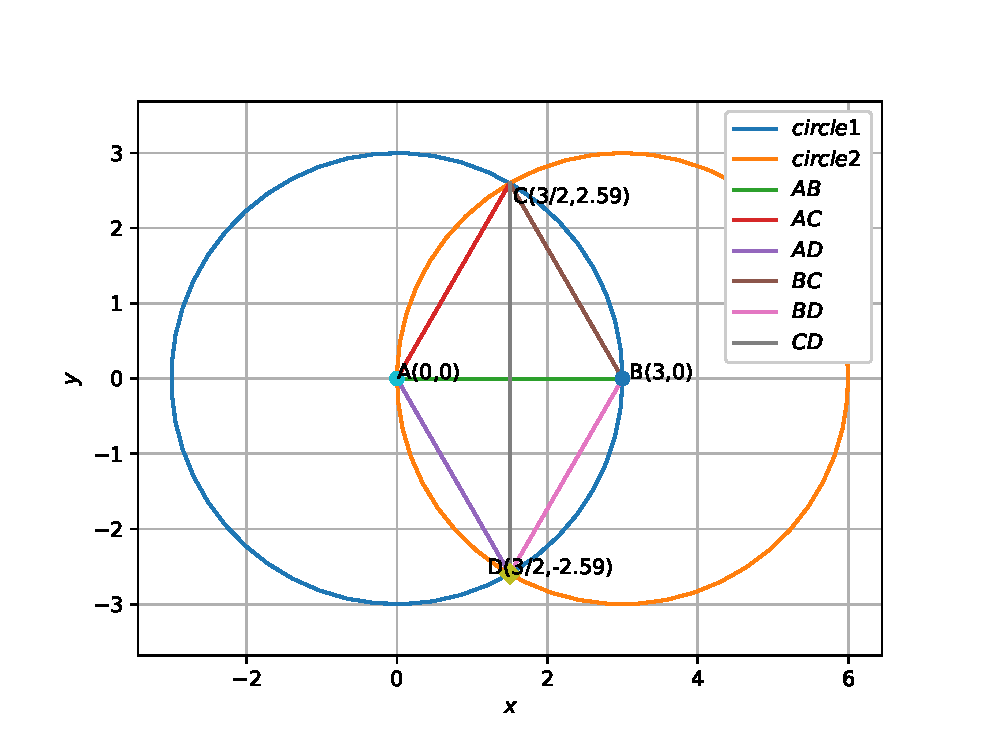
\includegraphics[width=0.8\columnwidth]{./figs/circle_con.eps}
	\end{center}
	\caption{Intersection of circles}
	\label{}	
\end{figure}
\end{frame}
\begin{frame}
\begin{figure}[!ht]
	\begin{center}
		\resizebox{0.8\columnwidth}{!}{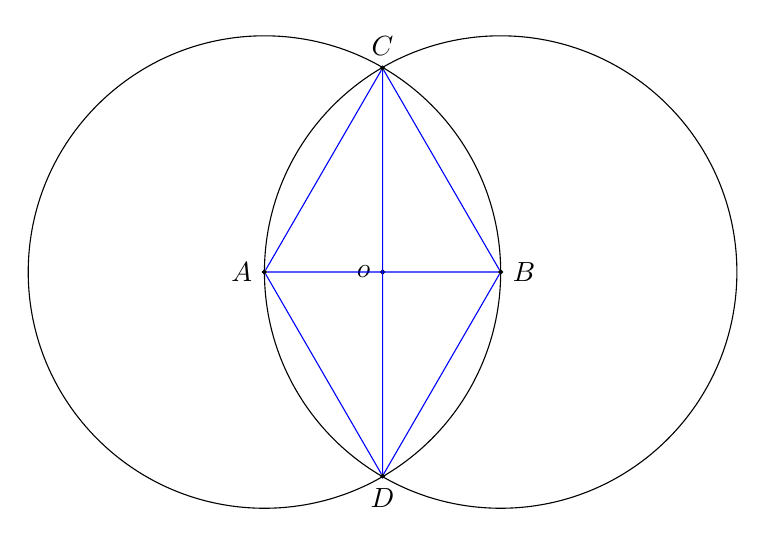
\begin{tikzpicture}
[scale=1,>=stealth,point/.style={draw,circle,fill = black,inner sep=0.5pt},]
%Inradius
\def\r{3} 
\node (A) at (0,0)[point,label=left:$A$] {};
\def\s{3} 
\node (B) at (3,0)[point,label=right:$B$] {};

%Drawing circle
\color{black}
\draw (A) circle (\r);
\draw (B) circle (\s);

%intersecting points
\def\a{1.5}
\def\b{2.59}
\color{black}
\node (C) at (\a,\b)[point,label=above:$C$] {};
\node (D) at (\a,-\b)[point,label=below:$D$] {};
\node (o) at (\a,0)[point,label=left:$o$] {};

%Drawing Rhombus
\color{blue}
\draw (A) -- node[left] {$\textrm{}$} (B) -- node[below] {$\textrm{}$} (C) -- node[right,,xshift=2mm] {$\textrm{}$} (A)-- node[below] {$\textrm{}$} (D)-- node[below] {$\textrm{}$} (B) (D)-- node[below] {$\textrm{}$} (C);
%Drawing the angles
\tkzMarkRightAngle[fill=black!20,size=.3](C,o,B)
\tkzMarkRightAngle[fill=black!20,size=.3](C,o,A)
\tkzMarkRightAngle[fill=black!20,size=.3](D,o,B)
\tkzMarkRightAngle[fill=black!20,size=.3](D,o,A)
\end{tikzpicture}}
	\end{center}
	\caption{Intersection of circles}
	\label{}	
\end{figure}
\end{frame}
\begin{frame}
\textbf{Coordinates of Circle:}
\begin{enumerate}
\item Construct two circles A and B which are intersecting at C and D.
\item A = $\begin{pmatrix} 0\\0 \end{pmatrix}$ ,B = $\begin{pmatrix} 3\\0 \end{pmatrix}.$
\item C = $\begin{pmatrix} p\\q \end{pmatrix} = \begin{pmatrix} \frac{3}{2}\\2.59 \end{pmatrix}$ ,
D = $\begin{pmatrix} p\\-q \end{pmatrix} = \begin{pmatrix} \frac{3}{2}\\-2.59 \end{pmatrix}.$\\
p and q are given as p = $\frac{c^2+b^2-a^2}{2c}$ = $\frac{3}{2}$ and\\
 q = $\sqrt{b^2-p^2} = 2.59$ (where a = b = c =3).
\end{enumerate}
\url{https://github.com/Narendrapulipati/geometry/blob/master/codes/cir_con.py}
\url{https://github.com/Narendrapulipati/geometry/blob/master/figs/circle_con.tex}
\end{frame}